\section{LOGLOG Log-Log Plot Function}

\subsection{Usage}

This command has the exact same syntax as the \verb|plot| command:
\begin{verbatim}
  loglog(<data 1>,{linespec 1},<data 2>,{linespec 2}...,properties...)
\end{verbatim}
in fact, it is a simple wrapper around \verb|plot| that sets the
x and y axis to have a logarithmic scale.
\subsection{Example}

Here is an example of a doubly exponential signal plotted first on a linear
plot:
\begin{verbatim}
--> x = linspace(1,100);
--> y = x;
--> plot(x,y,'r-');
\end{verbatim}


\centerline{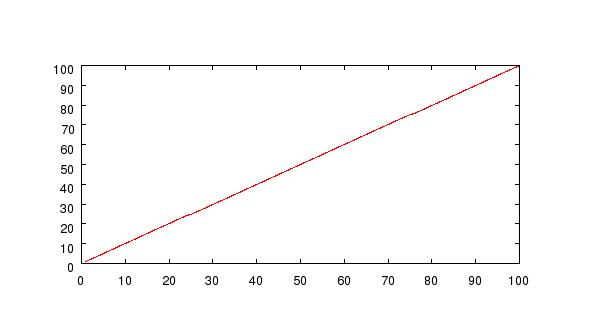
\includegraphics[width=8cm]{loglog1}}

and now on a log-log plot
\begin{verbatim}
--> loglog(x,y,'r-');
\end{verbatim}


\centerline{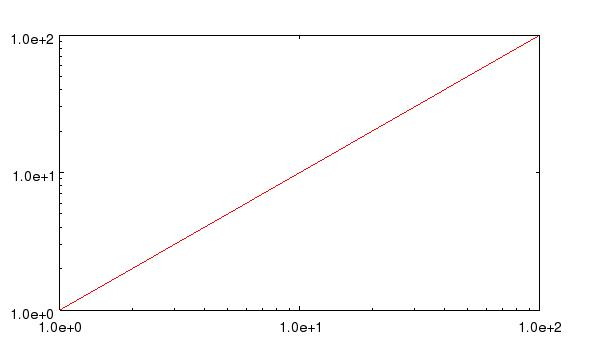
\includegraphics[width=8cm]{loglog2}}

